\documentclass{beamer}
\usepackage{graphicx}

\newcommand{\lp}{\left(}
\newcommand{\rp}{\right)}
\newcommand{\lb}{\left\{}
\newcommand{\rb}{\right\}}
\newcommand{\lf}{\left\lfloor}
\newcommand{\rf}{\right\rfloor}
\newcommand{\lc}{\left\lceil}
\newcommand{\rc}{\right\rceil}
\newcommand{\ls}{\left[}
\newcommand{\rs}{\right]}
\newcommand{\la}{\left|}
\newcommand{\ra}{\right|}
\newcommand{\lan}{\left\langle}
\newcommand{\ran}{\right\rangle}

\mode<presentation> {
  \usetheme{Rochester}
}

\usepackage{lmodern}

\title{Information Theory: Entropy}
\author{Herbert Ilhan Tanujaya}
\date{A0144892W}

\everymath{\displaystyle}

\begin{document}

\begin{frame}
  \titlepage
\end{frame}

\begin{frame}
  \frametitle{Definition}
  Let $X$ be a discrete random variable with probability distribution $p(x)$.
  \begin{block}{Entropy $H_X$}
    \[ H_X = - \sum_{x \in X} p(x) \log_2 p(x) = \mathbb{E} \log_2 \ls \frac{1}{p(X)} \rs. \]
  \end{block}
  Here we define $0 \log_2 0 = 0$.

  In a sense, the entropy of a random variable shows how ``surprising'' the event is.
\end{frame}

\begin{frame}
  \frametitle{Examples}
  \begin{exampleblock}{Entropy of a fair coin}
    A fair coin has entropy $\frac{1}{2} \log_2(2) + \frac{1}{2} \log_2(2) = 1$.
  \end{exampleblock}

  \begin{exampleblock}{Entropy of a fair $m$-sided die}
    A $m$-sided die has entropy $\log_2(m)$.
  \end{exampleblock}

  \begin{exampleblock}{Entropy of $n$ fair coin flips}
    Flipping $n$ coins produce $2^n$ uniformly distributed possibilities, and hence, the entropy is $n$.
  \end{exampleblock}
\end{frame}

\begin{frame}
  \frametitle{Examples}

  \begin{exampleblock}{Entropy of a Bernoulli trial}
    If $X$ is a random variable taking values between 0 and 1, where $p(0) = p$ and $p(1) = 1 - p$, its entropy is \[ H_p = -p \log_2 p - (1 - p) \log_2 (1 - p). \]

    \begin{center}
      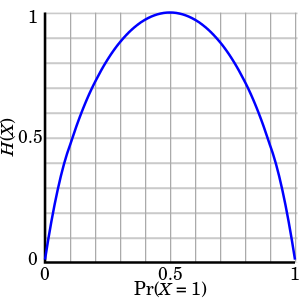
\includegraphics[width=3cm]{bernoulli.png}
    \end{center}
  \end{exampleblock}
\end{frame}

\begin{frame}
  \frametitle{Example}
  \begin{exampleblock}{Entropy of an unfair dice}
    An unfair dice with four faces and \[ p(1) = 1/2, p(2) = 1/4, p(3) = 1/8, p(4) = 1/8 \] has entropy $7/4$, smaller than the one of the corresponding fair dice $2$. (This dice is less surprising than the fair dice.)
  \end{exampleblock}
\end{frame}

\begin{frame}
  \frametitle{Motivation [TODO]}
  Define a function $H$ that takes in a random variable and outputs an integer, such that:
  \begin{itemize}
    \item If a random variable $X$ takes $n$ values, then $H(X)$ is maximized if $X$ is uniform.
    \item Entropy is additive, in the sense that: if $X$ takes $x_i$ with probability $p_i$, $Y$ takes $x_i$ with probability $q_i$, and $Z$ takes $x_i$ with probability $\alpha p_i + \beta q_i$ for all $i$, then \[ H(Z) = \alpha H(X) + \beta H(Y). \]
  \end{itemize}
  Then $H(X) = - \sum p_i \log p_i$ is the only possible function (up to the base of the logarithm).
\end{frame}

\begin{frame}
  \frametitle{Properties (TPM 15.7.1)}
  \begin{enumerate}
    \item $H(X) \le \log |S|$.
    \item $H(X) \le H(X, Y) \le H(X) + H(Y)$.
    \item $H(X|Y, Z) \le H(X|Y)$.
  \end{enumerate}

  \begin{block}{Entropy is subadditive (TPM 15.7.2)}
    Let $X = (X_1, \dotsc, X_n)$ be a random variable taking values in the set $S = S_1 \times S_2 \times \dotsb \times S_n$, where each of the coordinates $X_i$ of $X$ is a random variable taking values in $S_i$. Then \[ H(X) \le \sum_{i = 1}^n H(X_i). \] (This is just induction on the property $H(X, Y) \le H(X) + H(Y)$.)
  \end{block}
\end{frame}

\begin{frame}
  \frametitle{TPM 15.7.3}
  Let $\mathcal{F}$ be a family of subsets of $\{ 1, 2, \dotsc, n \}$ and let $p_i$ denote the fraction of sets in $\mathcal{F}$ that contain $i$. Then \[ |\mathcal{F}| \le 2^{\sum H(p_i)}. \]

  \begin{block}{Proof}
    Let $X = (X_1, \dotsc, X_n)$ taking $F \in \mathcal{F}$ with equal probability. Then $H(X) \le \sum H(X_i)$ implies $\log |\mathcal{F}| \le \sum H(p_i)$.
  \end{block}
\end{frame}

\begin{frame}
  \frametitle{TPM 15.7.4}
  Let $X = (X_1, \dotsc, X_n)$ taking values in $S = S_1 \times \dotsb \times S_n$, where each $X_i$ takes values in $S_i$. For an index set $I \subseteq \{ 1, 2, \dotsc, n \}$ let $X(I)$ denote $(X_i)_{i \in I}$. If $\mathcal{G}$ is a family of subsets of $\{ 1, \dotsc, n \}$ and each $i \in \{ 1, \dotsc, n \}$ belongs to at least $k$ members of $\mathcal{G}$, then \[ kH(X) \le \sum_{G \in \mathcal{G}} H(X(G)). \]

  \begin{block}{Proof}
    Use induction. If there is $G \in \mathcal{G}$ where $G = \{ 1, \dotsc, n \}$ we are done. Otherwise, we prove \[ H(X(G \cup G')) + H(X(G \cap G')) \le H(X(G)) + H(X(G')). \]
  \end{block}
\end{frame}

\begin{frame}
  \frametitle{TPM 15.7.5}
  Let $\mathcal{F}$ be a family of vectors in $S_1 \times S_2 \times \dotsb \times S_n$. Let $\mathcal{G} = \{ G_1, G_2, \dotsc, G_m \}$ be a collection of subsets of $N = \{ 1, 2, \dotsc, n \}$, and suppose that each element $i \in N$ belongs to at least $k$ members of $\mathcal{G}$. For each $1 \le i \le m$ let $\mathcal{F}_i$ be the set of all projections of the members of $\mathcal{F}$ on $G_i$. Then \[ |\mathcal{F}|^k \le \prod_{i = 1}^m |\mathcal{F}_i|. \]

  \begin{block}{Proof}
    Let $X = (X_1, \dotsc, X_n)$ taking $F \in \mathcal{F}$ with equal probability. Then $kH(X) \le \sum H(X(G_i))$ implies $k \log |\mathcal{F}| \le \sum \log |\mathcal{F}_i|$.
  \end{block}
\end{frame}
\end{document}
